\documentclass[11pt, dvipsnames, handout]{beamer}
\newtoggle{full}
\settoggle{full}{true}

\newtoggle{covered}
\settoggle{covered}{false}

\newtoggle{presentable}
\settoggle{presentable}{false}

\newtoggle{dualscreen}
\settoggle{dualscreen}{false}

\usepackage{pgfplots}
%\pgfplotsset{compat = newest}

\usepackage{pgfpages}

\setbeamertemplate{note page}{\pagecolor{yellow!5}\vfill \insertnote \vfill}
\usepackage{collect}
\definecollection{notes}
\newcounter{notestaken}

\usepackage{xpatch}

\usepackage{ulem}

\usepackage[framemethod=tikz]{mdframed}

\usepackage{scalerel}
\usepackage{calc}

%\usepackage{enumitem}
\setlength\fboxsep{.2em}

\usepackage{graphicx} % Allows including images
\usepackage{booktabs} % Allows the use of \toprule, \midrule and \bottomrule in tables

\xpatchcmd{\itemize}
  {\def\makelabel}
  {\setlength{\itemsep}{0.65 em}\def\makelabel}
  {}
  {}


\xpatchcmd{\beamer@enum@}
  {\def\makelabel}
  {\setlength{\itemsep}{0.65 em}\def\makelabel}
  {}
  {}


%\makeatletter
%\renewcommand{\itemize}[1][]{%
%  \beamer@ifempty{#1}{}{\def\beamer@defaultospec{#1}}%
%  \ifnum \@itemdepth >2\relax\@toodeep\else
%    \advance\@itemdepth\@ne
%    \beamer@computepref\@itemdepth% sets \beameritemnestingprefix
%    \usebeamerfont{itemize/enumerate \beameritemnestingprefix body}%
%    \usebeamercolor[fg]{itemize/enumerate \beameritemnestingprefix body}%
%    \usebeamertemplate{itemize/enumerate \beameritemnestingprefix body begin}%
%    \list
%      {\usebeamertemplate{itemize \beameritemnestingprefix item}}
%      {%
%        \setlength\topsep{1em}%NEW
%        \setlength\partopsep{1em}%NEW
%        \setlength\itemsep{1em}%NEW
%        \def\makelabel##1{%
%          {%
%            \hss\llap{{%
%                \usebeamerfont*{itemize \beameritemnestingprefix item}%
%                \usebeamercolor[fg]{itemize \beameritemnestingprefix item}##1}}%
%          }%
%        }%
%      }
%  \fi%
%  \beamer@cramped%
%  \raggedright%
%  \beamer@firstlineitemizeunskip%
%}
%
%
%
%
%
%\makeatother

%\setlist[beamer@enum@]{topsep=1 em}
%\let\origcheckmark\checkmark %screw you dingbat
%\let\checkmark\undefined %screw you dingbat
%\usepackage{dingbat} 
%\let\checkmark\origcheckmark %screw you dingbat






%\usepackage{fontawesome}

\usepackage{mathtools}
\usepackage{etoolbox, calculator}

\usepackage{xcolor}
\usepackage{tikz}
\usetikzlibrary{arrows.meta}
\usetikzlibrary{calc}
\usepackage[nomessages]{fp}
\usepackage{transparent}
\usepackage{accsupp}
%\usepackage{color, xcolor}

%colorblind-friendly palette
%\definecolor{dblue}{RGB}{51,34,136}
\definecolor{lblue}{RGB}{136,204,238}
%\definecolor{green}{RGB}{17,119,51}
\definecolor{tan}{RGB}{221,204,119}
%\definecolor{mauve}{RGB}{204,102,119}

\usepackage{tcolorbox}



\usepackage{xifthen}
\usepackage{nicefrac}
\usepackage{amsmath}
\usepackage{amsthm}
\usepackage{amssymb}
\theoremstyle{definition}
\newtheorem*{define}{Definition}
\newtheorem*{recall}{Recall}


\DeclareMathOperator{\tr}{tr}

\usepackage{multicol}
%\setlength{\columnsep}{1cm}

\usepackage{tablists, amsmath,vwcol, cancel, polynom}
\usetikzlibrary{shapes, patterns, decorations.shapes}
%\usepackage{tikzpeople}
\tikzstyle{vertex}=[shape=circle, minimum size=2mm, inner sep=0, fill]
\tikzstyle{opendot}=[shape=circle, minimum size=2mm, inner sep=0, fill=white, draw]

% common math quick commands
\newcommand{\nicedd}[2]{\nicefrac{\text{d}#1}{\text{d}#2}}
\newcommand{\dd}[2]{\dfrac{\text{d}#1}{\text{d}#2}}
\newcommand{\pd}[2]{\dfrac{\partial #1}{\partial#2}}
\renewcommand{\d}[1]{\text{d}#1}
\newcommand{\ddn}[3]{\dfrac{\text{d}^{#3}#1}{\text{d}#2^{#3}}}
\newcommand{\pdn}[3]{\dfrac{\partial^{#3}#1}{\partial#2^{#3}}}
\newcommand{\p}[0]{^{\prime}}
\newcommand{\pp}[0]{^{\prime\prime}}
\newcommand{\op}[2][\text{L}]{#1 \left[ #2 \right]}

\newcommand{\lap}[1]{\mathcal{L}\left\{#1\right\}}
\newcommand{\lapinv}[1]{\mathcal{L}^{-1}\left\{#1\right\}}
\newcommand{\lapint}[1]{\int_0^\infty e^{-st}#1dt}
\newcommand{\evalat}[2]{\Big|_{#1}^{#2}}

\newcommand{\paren}[1]{ \left( #1 \right)}

\newcommand{\haxis}[4][\normcolor]{\draw[#1, <->] (-#2,0)--(#3,0) node[right]{$#4$}; }


\newcommand{\axis}[4]{\draw[\normcolor, <->] (-#1,0)--(#2,0) 
node[right]{$x$};
\draw[help lines, <->] (0,-#3)--(0,#4) node[above]{$y$};}

\newcommand{\laxis}[6]{\draw[<->] (-#1,0)--(#2,0) 
node[right]{$#5$};
\draw[ <->] (0,-#3)--(0,#4) node[above]{$#6$};}
\newcommand{\xcoord}[2]{
	\draw (#1,.2)--(#1,-.2) node[below]{$#2$};}
\newcommand{\textnode}[3]{
	\draw (#1,#2) node[below]{$#3$};}
	
\newcommand{\nxcoord}[2]{
	\draw (#1,-.2)--(#1,.2) node[above]{$#2$};}
\newcommand{\ycoord}[2]{
	\draw (.2,#1)--(-.2,#1) node[left]{$#2$};}
\newcommand{\nycoord}[2]{
	\draw (-.2,#1)--(.2,#1) node[right]{$#2$};}
\newcommand{\dlim}{\displaystyle\lim}
\newcommand{\dlimx}[1]{\displaystyle\lim_{x \rightarrow #1}}
\newcommand{\stickfig}[2]{
	\draw (#1,#2) arc(-90:270:2mm);
	\draw (#1,#2)--(#1,#2-.5) (#1-.25,#2-.75)--(#1,#2-.5)--(#1+.25,#2-.75) (#1-.2,#2-.2)--(#1+.2,#2-.2);}	

%\newcounter{example}
%\setcounter{example}{1}
%\newcounter{preFrameExample}
%\AtBeginEnvironment{frame}{\setcounter{preFrameExample}{\value{example}}}
%\newcommand{\ex}[1]{
%	 \setcounter{example}{\value{preFrameExample}}
%	 \textcolor{green}{\small\fbox{Example \arabic{example}: #1}}\\[8pt]
%	\stepcounter{example}}
%\newcommand{\exans}[1]{
%	\SUBTRACT{\value{preFrameExample}}{1}{\n}
%	 \textcolor{green}{\small\fbox{Solution \n: #1}}\\[8pt]}
\mode<presentation> {

% The Beamer class comes with a number of default slide themes
% which change the colors and layouts of slides. Below this is a list
% of all the themes, uncomment each in turn to see what they look like.


\usetheme{CambridgeUS}
\usecolortheme[named=black]{structure}


\newcommand{\studentcolor}[0]{ForestGreen}
\newcommand{\normcolor}[0]{NavyBlue}
\newcommand{\alertcolor}{Red}

\setbeamercolor{normal text}{fg=\normcolor}
\setbeamercolor{frametitle}{fg=\normcolor}
\setbeamercolor{section in head/foot}{fg=Black, bg=Gray!20}
\setbeamercolor{subsection in head/foot}{fg=Green!70!Black, bg=Gray!10}
\setbeamercolor{alerted text}{fg=\alertcolor}
\setbeamerfont{alerted text}{series=\bf}
\setbeamertemplate{enumerate items}[default]
\setbeamercolor{enumerate item}{fg=\normcolor}

\setbeamertemplate{footline} % To remove the footer line in all slides uncomment this line
%\setbeamertemplate{footline}[page number] % To replace the footer line in all slides with a simple slide count uncomment this line

\setbeamertemplate{navigation symbols}{} % To remove the navigation symbols from the bottom of all slides uncomment this line
}

\newcommand{\alertbox}[1]{\tcbox[on line, colframe=\alertcolor, colback=White, left=2pt,right=2pt,top=2pt,bottom=2pt]{\usebeamercolor*{normal text}#1}}


\newcommand{\startstu}{\setbeamercolor{normal text}{fg=\studentcolor}\usebeamercolor*{normal text}\setbeamercolor{enumerate item}{fg=\studentcolor}\usebeamercolor*{enumerate item}}
\newcommand{\stopstu}{\setbeamercolor{normal text}{fg=\normcolor}\usebeamercolor*{normal text}\setbeamercolor{enumerate item}{fg=\normcolor}\usebeamercolor*{enumerate item}}

\newcommand{\takenote}[1]{ \begin{collect}{notes}{}{}{}{}  #1  \end{collect}  \addtocounter{notestaken}{1}} %\ifthenelse{\value{notestaken}>0}{\hrulefill\\}{}

\makeatletter
\newcommand{\cover}{\alt{\beamer@makecovered}{\beamer@fakeinvisible}}
\newcommand{\ucover}[1]{\iftoggle{full}{}{\beamer@endcovered}\stopstu#1\startstu\iftoggle{full}{}{\beamer@startcovered}}
\makeatother

\newcommand{\skippause}{ \addtocounter{beamerpauses}{-1}}
\newcommand{\blockpres}{ \skippause \pause }

\newcommand{\studentify}[1]{\startstu #1  \stopstu }
\newcommand{\student}[1]{\iftoggle{full}{ \pause  \studentify{#1} }{\iftoggle{covered}{\studentify{#1}}{\cover{  #1 }}}}
\newcommand{\cstudent}[1]{\student{\begin{center} #1 \end{center}}}
\newcommand{\fullonly}[1]{\iftoggle{full}{ #1}{}}
\newcommand{\presentonly}[1]{\iftoggle{presentable}{ #1}{}}

\usepackage{xparse}
\usepackage{xifthen}

% shortcuts for commonly-used presentation elements
%\NewDocumentCommand{\slide}{o m}
% {\IfValueTF{#1}{\begin{frame}[t]{#1}}{\begin{frame}[t]} #2 \end{frame}}

\newtoggle{iscovered}

\newcommand{\slide}[2][]{%
%\setcounter{notestaken}{0}
\takenote{#2} 
%\ifthenelse{\equal{#1}{}}{\begin{frame}[t]}{\begin{frame}[t]{#1}} #2 \ifthenelse{\value{notestaken}>0}{ \note{\includecollection{notes}}}{} \end{frame}%
\ifthenelse{\equal{#1}{}}{\begin{frame}[t]}{\begin{frame}[t]{#1}} #2 \iftoggle{covered}{\settoggle{iscovered}{true}}{\settoggle{iscovered}{false}}  \note{ \iftoggle{iscovered}{}{\settoggle{covered}{true}} #2 \iftoggle{iscovered}{}{\settoggle{covered}{false}} } \end{frame}%
%\setcounter{notestaken}{0}
}
\newcommand{\defn}[2][]{%
 \setcounter{listcounter}{0}%
\ifthenelse{\equal{#1}{}}{\begin{block}{Definition}}{\begin{block}{#1 :}}%
 #2 \vspace{0.25em} \ifthenelse{\value{listcounter}>0}{\skippause}{} \pause \end{block}%
}



\newcommand{\arr}[2]{\begin{array}{#1}#2\end{array}}
\newcommand{\mat}[2]{\left[\arr{#1}{#2}\right]}
\newcommand{\carray}[1]{\arr{c}{#1}}
\newcommand{\larray}[1]{\arr{l}{#1}}
\newcommand{\rarray}[1]{\arr{r}{#1}}
\newcommand{\colvec}[1]{\mat{c}{#1}}

\newcommand{\itmz}[1]{\addtocounter{listcounter}{1} \begin{itemize}#1 \end{itemize} }
\newcommand{\subitem}[1]{\addtocounter{listcounter}{1} \begin{itemize} \item #1 \end{itemize}}
%
\newcommand{\enum}[1]{\addtocounter{listcounter}{1} \begin{enumerate} #1  \end{enumerate}  }


\newcommand{\algnlbl}[1]{\begin{align}#1  \end{align}} 
\newcommand{\algn}[1]{\begin{align*}#1  \end{align*}} 
\newcommand{\lgn}[1]{ \action<+->{#1} }
\newcommand{\slgn}[1]{\iftoggle{full}{\action<+->{ \startstu #1 \stopstu}}{ \cover{ #1 } } \takenote{$#1$}}

\newcommand{\chckmrk}{\alert{\checkmark}}

\usepackage{pifont}
\newcommand{\xmark}{\alert{\text{\large \ding{55}}}}

\newcommand{\return}[0]{\raisebox{.5ex}{\rotatebox[origin=c]{180}{$\Lsh$}}}
\usepackage{pbox}
%\newcommand{\ex}[1]{\rotatebox[origin=c]{10}{\uline{ex}}:$\;$\pbox[t][][b]{0.9\linewidth}{#1}}
\newcommand{\ex}[1]{\uline{ex}:$\;$\pbox[t][][t]{0.9\linewidth}{#1}}
\newcommand{\eg}[1]{e.g.,$\;$\pbox[t][][t]{0.9\linewidth}{#1}}
\newcommand{\tikzplot}[8][]{%
\begin{tikzpicture}

\begin{scope}[]%
\clip(-#2,-#4) rectangle (#3,#5);%
#8%
\end{scope}%
\laxis{#2}{#3}{#4}{#5}{#6}{#7}%
#1
\end{tikzpicture}%
}


\newcommand{\cancelslide}[1]{%
\begingroup%
\setbeamertemplate{background canvas}{%
\begin{tikzpicture}[remember picture,overlay]%
\draw[line width=2pt,red!60!black] %
  (current page.north west) -- (current page.south east);%
\draw[line width=2pt,red!60!black] %
  (current page.south west) -- (current page.north east);%
\end{tikzpicture}}%
#1%
\endgroup%
}
\renewcommand{\CancelColor}{\color{red}}
\newcommand{\twocols}[3][0.5]{\begin{columns}\begin{column}{#1\textwidth}#2\end{column}\hspace{1em}\vrule{}\hspace{1em}\begin{column}{#1\textwidth}#3\end{column}\end{columns}}

\newcommand{\twomini}[5][1]{\calculatespace \begin{minipage}[t]{\columnwidth}\begin{minipage}[][#1\contentheight][t]{#2\columnwidth}#4\end{minipage}\hfill\begin{minipage}[][#1\contentheight][t]{#3\columnwidth}#5\end{minipage}\end{minipage}}

\newcommand{\threemini}[7][1]{\calculatespace \begin{minipage}[t]{\columnwidth}\begin{minipage}[][#1\contentheight][t]{#2\columnwidth}#5\end{minipage}\hfill\begin{minipage}[][#1\contentheight][t]{#4\columnwidth}#6\end{minipage}\hfill\begin{minipage}[][#1\contentheight][t]{#3\columnwidth}#7\end{minipage}\end{minipage}}


\newcounter{listcounter}
\setcounter{listcounter}{0}



\newif\ifsidebartheme
\sidebarthemetrue

\newdimen\contentheight
\newdimen\contentwidth
\newdimen\contentleft
\newdimen\contentbottom
\makeatletter
\newcommand*{\calculatespace}{%
\contentheight=\paperheight%
\ifx\beamer@frametitle\@empty%
    \setbox\@tempboxa=\box\voidb@x%
  \else%
    \setbox\@tempboxa=\vbox{%
      \vbox{}%
      {\parskip0pt\usebeamertemplate***{frametitle}}%
    }%
    \ifsidebartheme%
      \advance\contentheight by-1em%
    \fi%
  \fi%
\advance\contentheight by-\ht\@tempboxa%
\advance\contentheight by-\dp\@tempboxa%
\advance\contentheight by-\beamer@frametopskip%
\ifbeamer@plainframe%
\contentbottom=0pt%
\else%
\advance\contentheight by-\headheight%
\advance\contentheight by\headdp%
\advance\contentheight by-\footheight%
\advance\contentheight by4pt%
\contentbottom=\footheight%
\advance\contentbottom by-4pt%
\fi%
\contentwidth=\paperwidth%
\ifbeamer@plainframe%
\contentleft=0pt%
\else%
\advance\contentwidth by-\beamer@rightsidebar%
\advance\contentwidth by-\beamer@leftsidebar\relax%
\contentleft=\beamer@leftsidebar%
\fi%
}
\makeatother


\iftoggle{dualscreen}{\setbeameroption{show notes on second screen=right}}{}

\usepackage{circuitikz}

\begin{document}
\section{Lecture 4+5}
\subsection{Introduction}
\slide[Review]{
Linear First Order DE:\[ y\p+p(t)y=g(t)\]\vspace{-1em}
\student{\[ \underbrace{y_h\p+p(t)y_h=0}_{\text{Homogeneous Problem}}\]}\vfill
Linearity $\Rightarrow$ General Solution Structure:
\[y_g =\underbrace{ \underbrace{y_p}_{\student{\carray{\textbf{Particular Part} \\ \text{-} \\ \text{Method of Undetermined Coefficients}}}} + \underbrace{y_h}_{\student{\carray{\textbf{Homogeneous Part} \\ \text{-} \\ \text{General Solution}}}}}_{\student{\text{Method of Integrating Factors}}}\]
\vfill
\student{What happens when we add in $y\pp$}
}

\slide[Overview]{
Second order linear differential equations
\itmz{
\item  Where do these DEs arise?
\item Existence \& uniqueness of solutions
\item Superposition again:
\subitem{General solution = homogeneous solution + particular solution}
}
}


\slide[Spring-dashpot system:]{
\twomini[.6]{.35}{.65}{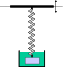
\includegraphics[width=\columnwidth]{images/spring_dashpot.pdf}}{\vfill
$x(t)=$ displacement from rest position\\
$f(t)=$ applied force
\vfill
Newton's 2$^{nd}$ Law:
\algn{ F &= ma\\
 - kx - \beta \dd{x}{t} +f(t) &= m\ddn{x}{t}{2}}\vspace*{\fill} }
\vfill
\centerline{\includegraphics[width=.3\columnwidth]{images/sin_graph.pdf}\hfill\includegraphics[width=.3\columnwidth]{images/sin_exp_graph.pdf}\hfill
\includegraphics[width=.3\columnwidth]{images/exp_graph.pdf}}
}


\slide[Torsional motion of a weight on a twisted shaft:]{
\twomini{.32}{.65}{
\includegraphics[width=\columnwidth]{images/twisted_shaft.pdf}}{
\vfill\[ I\ddn{\theta}{t}{2} +c \dd{\theta}{t} + k\theta = T(t)\]\vspace*{\fill}
}
}

\slide[L-R-C series circuits:]{
\twomini{.45}{.55}{
\begin{circuitikz} \draw
       (0,-1.5)   to[vsourcesin, l=\textcolor{black}{$E(t)$}] (0,1.5)
	[black] -- (0.5,1.5)
        to[L, l=$L$, black] (1.5,1.5) -- (2.5,1.5)
        to[C, l=$C$, black] (2.5,0) -- (2.5,-1.5)
        to[R, l=$R$, black] (.5,-1.5) -- (0,-1.5) ;
    \end{circuitikz}
}{\vfill
Q=charge on capacitor\\~\\
$\dd{Q}{t}$=current in circuit\\~\\
$E(t)$ = applied voltage\\
\vfill
Kirchoff's Laws:
\[ L\ddn{Q}{t}{2} +R \dd{Q}{t} + \frac1CQ = E(t)\]\vspace*{\fill}
}
}

\slide[Small oscillations of a pendulum:]{
\twomini{.45}{.55}{\includegraphics[width=\columnwidth]{images/pendulum.pdf}}{
\vfill\[ mL^2\ddn{\theta}{t}{2}=-cL \dd{\theta}{t} -mgL\theta + F(t) \]\vspace*{\fill}
}
}

\slide[Equivalence of Problems]{
These 4 physical systems are modelled identically by:\[Ay\pp+By\p+Cy=D(t)\]
\vfill
Constants have different physical meaning (\& units)
\small\vfill
\begin{tabular}{|>{\centering}m{2cm}|>{\centering}m{2cm}|>{\centering}m{2cm}|>{\centering}m{2cm}|>{\centering}p{2cm}|}
\hline 
\textbf{System} & \textbf{A} & \textbf{B} & \textbf{C} & \textbf{D}\tabularnewline
\hline 
\hline 
\textbf{Spring Dashpot} & Mass & Damping Coeff. & Spring Constant & Applied Force\tabularnewline
\hline 
\textbf{Pendulum} & Mass x (Length)$^{2}$ & Damping x Length & Gravitational Moment & Applied Moment\tabularnewline
\hline 
\textbf{Series Circuit} & Inductance & Resistance & Capacitance$^{-1}$ & Imposed Voltage\tabularnewline
\hline 
\textbf{Twisted Shaft} & Moment of Inertia & Damping & Elastic Shaft Constant & Applied Torque\tabularnewline
\hline 
\end{tabular}

}

\slide[General Linear 2nd Order DE’s]{
\begin{equation}
\ddn{y}{t}{2} + p(t)\dd{y}{t} +q(t)y=g(t)  \label{eq:ODE}
\end{equation}

\itmz{\item $g(t)$ represents the "forcing" term, an external influence.
\student{\subitem{Homogeneous if $g(t)=0$ for all $t \in I$ \item Inhomogeneous if $g(t)\neq0$ for all $t\in I$}}\vfill
\item $p(t)$ and $q(t)$ represent the intrinsic properties of the physical system.
\student{\subitem{Often consant, but not always \item e.g., an aging spring could be modelled by $q=q(t)$.}}\vfill
\item Solution to \eqref{eq:ODE} is defined on an interval $t\in I=(\alpha,\beta)$
}
}
\subsection{IVP Solutions}
\slide[Initial Conditions]{
IVP = Initial Value Problem
\student{\subitem{Consists of Eq. \eqref{eq:ODE} plus a set of initial conditions:
\begin{equation} y(t_0)=y_0, \quad y\p(t_0)=v_0 \label{eq:IC}\end{equation}}
}
\vfill
Why are there two initial conditions?
\student{\subitem{2nd order $\Rightarrow$ integrate twice to solve $\Rightarrow$ two constants of integration \\ \centerline{$\Downarrow$} \centerline{Need two initial conditions for a well-defined solution}}}
}

\slide[Existence and uniqueness of solutions]{
\textbf{Theorem 1:} Consider the IVP \algn{\ddn{y}{t}{2} + p(t)\dd{y}{t} +q(t)y&=g(t), &t\in I\\
y(t_0)=y_0,\quad y\p(t_0)&=v_0,&t_0\in I}  where $p(t)$, $q(t)$, and $g(t)$ are \textbf{continuous} for $t\in I = (\alpha, \beta)$
\\~\\
There is a single solution to this IVP, and the solution is defined throughout the time interval $I$
\vfill
\textbf{Notes: } \student{Discontinuities create kinks or jumps in the solution.
\tikzplot[
\student{\xcoord{3}{\text{kink}} }
]{.1}{5}{.1}{1.5}{t}{}{
\student{
\draw[domain=0:2, thick, samples=100] plot ({\x*1.5}, {.8*exp(-\x)});
\draw[domain=2:10, thick, samples=100] plot ({\x*1.5}, {.8*exp(-\x)+(1-exp(-(\x-2)))*1.25});

}}\hfil \tikzplot[
\student{\xcoord{3}{\text{jump}} }
]{.1}{5}{.1}{1.5}{t}{}{
\student{
\draw[domain=0:2, thick, samples=100] plot ({\x*1.5}, {.8*exp(-\x)});
\draw[domain=2:10, thick, samples=100] plot ({\x*1.5}, {.8*exp(-(\x-2))});
\draw[thick , dashed] (3,0.1)--(3,.8);
}}
}\vfill 


}

\slide[Superposition Principle]{
\textbf{Theorem 2:} Suppose $y_1$ and $y_2$ are solutions to 
\algn{\ddn{y_1}{t}{2} + p(t)\dd{y_1}{t} +q(t)y_1&=g_1(t), &t\in I\\
\ddn{y_2}{t}{2} + p(t)\dd{y_2}{t} +q(t)y_2&=g_2(t), &t\in I. }\\~\\
Then, for any values of the constants $c_1$ and $c_2$, the linear combination $y=c_1y_1+c_2y_2$ satisifes \algn{\ddn{y}{t}{2} + p(t)\dd{y}{t} +q(t)y&=c_1g_1(t)+c_2g_2(t), &t\in I.}
}

\slide[Solution Structure]{
\algnlbl{\ddn{y}{t}{2} + p(t)\dd{y}{t} +q(t)y&=g(t)  &\nonumber\eqref{eq:ODE}\\
 y(t_0)=y_0, \quad y\p(t_0)&=v_0 &\nonumber \eqref{eq:IC}\\
\ddn{y}{t}{2} + p(t)\dd{y}{t} +q(t)y&=0 \label{eq:homoODE}
}\\~\\
\[\underbrace{\quad y_g(t) \quad}_{\carray{\textbf{General} \\ \text{Solution} \\ \text{of \eqref{eq:ODE}}}} \quad = \quad \underbrace{\quad y_p(t) \quad}_{\carray{\textbf{Particular} \\ \text{Solution} \\ \text{of \eqref{eq:ODE}}}} \qquad+ \underbrace{\qquad y_c(t) \qquad}_{\carray{\text{Particular solution of \eqref{eq:homoODE} + \eqref{eq:IC}}\\ = \\ \text{\textbf{Complementary} part}}}  \]
}

\slide[Homogeneous Solution Structure]{
\student{
\algn{\intertext{1$^{st}$ Order DE:} y\p +q(t)y&=0\\
\Rightarrow y_h &= c_1 y_1\\
ex.\quad  p(t)=a \Rightarrow y_h&=Ce^{-at}
\intertext{2$^{nd}$ Order DE:} y\pp+p(t)y\p +q(t)y&=0\\
\Rightarrow y_h &=c_1 y_1 + c_2 y_2\\
}\vfill
Both $y_1$ and $y_2$ make the LHS=0, \uline{independently}.
}
}

\slide[How to construct $y_c$]{

 We need $y_h$ to satisfy \eqref{eq:homoODE} and the two initial values (\ref{eq:IC})
\algn{y(t_0) = y_0, \quad y\p(t_0)&=v_0 &(\ref{eq:IC})\\ \ddn{y}{t}{2} + p(t)\dd{y}{t} +q(t)y&=0 &\eqref{eq:homoODE}}
\student{\[ y_h = c_1 y_1 + c_2 y_2\]\vfill
\centerline{Do some algebra to solve for $c_1$ and $c_2$.}\vfill
\centerline{Is the algebra  always possible?}}
}



\slide[]{Can we always satisfy (\ref{eq:IC}) with $c_1y_1+c_2y_2$?
\subitem{If so, then $y=c_1y_1+c_2y_2$ is the general solution of \eqref{eq:homoODE}} 
\student{\algn{c_1 y_1 +c_2 y_2 &= y_0\\c_1y_1\p+c_2y_2\p&=v_0 \intertext{Express in matrix notation}  \mat{cc}{y_1&y_2\\y_1\p&y_2\p} \mat{c}{c_1\\c_2} &= \mat{c}{y_0\\v_0}\\   A \quad\qquad x \quad &=  \quad b\\
\text{Solution:} \qquad x&=A^{-1}b &\text{if $A^{-1}$ exists}
}

Under what conditions does the matrix $A^{-1}$ exist?\\~\\ \centerline{$\det A \neq 0$}
}
}
\subsection{The Wronskian}
\slide[Wronskian Determinant]{
For two differentiable functions, $y_1(t)$ and $y_2(t)$, the Wronskian determinant is denoted $W\left(y_1, y_2\right)(t)$, and is defined by 
\[ W\left(y_1, y_2\right)(t) = \left| \begin{array}{cc} y_1(t)&y_2(t)\\y_1\p(t)&y_2\p(t) \end{array} \right| = y_1(t)y_2\p(t)-y_2(t)y_1\p(t)\]

\student{\subitem{$W\left(y_1, y_2\right)(t_0)\neq0$ is the condition that allows $c_1y_1+c_2y_2$ to satisfy ANY initial conditions at $t_0$.}}
\vfill
A set of 2 solutions, $y_1(t)$ and $y_2(t)$ , to  Eq. \eqref{eq:homoODE} on the
time interval $I$, is called a \textbf{fundamental set of solutions} if
$W\left(y_1, y_2\right)(t)\neq0$ for some $t \in I$:
\[y_c=c_1y_1+c_2y_2\]
}
\subsection{Fundamental sets of solutions}
\slide[Generality of Fundamental Solutions]{\vspace{-1em}
For 2 solutions $y_1(t)$ and  $y_2(t)$ of Eq. \eqref{eq:homoODE} on $I$, show that if $W\left( y_1,y_2 \right)(t) \neq 0$ for for some $t_0\in I$, then in fact $W\left( y_1,y_2 \right)(t) \neq 0$ for all $t \in I$.\\
\student{$y\pp+p(t)y\p+q(t)y=0 \qquad \Rightarrow \qquad y\pp=-p(t)y\p-q(t)y$
\algn{W&=y_1y_2\p-y_1\p y_2 \\
\dd{W}{t} &=\cancel{y_1\p y_2\p} + y_1 y_2\pp -y_1\pp y_2-\cancel{y_1\p y_2\p}\\
&= y_1 \left[-p(t)y_2\p-q(t)y_2\right] -   \left[-p(t)y_1\p-q(t)y_1\right]  y_2 \\
&= -p(t)y_1y_2\p-\cancel{q(t)y_1y_2} + p(t)y_1\p  y_2  + \cancel{q(t)y_1 y_2 } \\
&= -p(t)y_1y_2\p +  p(t)y_1\p  y_2 = -p(t) \left[ y_1y_2\p-y_1\p y_2  \right] \\
W\p &= - p(t) W
}\vfill
We can solve $W\p+p(t)W=0$ using the method of integrating factors!
}
}

\slide[]{\student{$W\p+p(t)W=0 \qquad \Rightarrow \qquad \mu = e^{\intop p(t)dt}$
\algn{\mu(t) W(t) &= \int 0 dt + C\\
W(t) & = \frac{C}{\mu(t)} & \Rightarrow W(t)&= C e^{-\int p(t)dt}\\
\intertext{Assuming the integral of $p(t)$ is finite, we have two cases:}
}\vspace{-3em}
\enum{\item $C=0 \qquad \Rightarrow W(t)=0$ for all $t$
\item $C\neq 0 \qquad \Rightarrow W(t)\neq0$ for all $t$}
\vfill
Suppose that at some $t_0$ we find that  $W(t_0)\neq0$ \[\Rightarrow  C\neq0 \Rightarrow W(t)\neq0 \quad  \text{for all t}\]
}

}

\slide[Linear dependence of functions]{
\itmz{
\item Two functions $f$ and $g$ are \textbf{linearly dependent} on $I=(\alpha,\beta)$ if there exist constants $k_1$and $k_2$ , not both zero,
such that \[k_1f+k_2g = 0 \quad \forall t\in I\] 
\vfill
\item The functions are \textbf{linearly independent} on $I$ if they are
not linearly dependent on $I$.
\vfill
\item Note that if $f$ and $g$ are differentiable functions:
\student{
\itmz{
\item  $W\left( f,g \right)(t_0) \neq 0$ \hfill $\Leftrightarrow$ \hfill $f$ \& $g$ are \uline{linearly independent}
on $I$.
\item $f$ \& $g$ are linearly dependent \hfill $\Rightarrow$ \hfill \uline{$W\left( f,g \right)(t) = 0$} .
\item but $W\left( f,g \right)(t) = 0$  \hfill $\cancel{\Rightarrow}$ \hfill  $f$ \& $g$ are linearly dependent
}
}
}
}

\slide[Summary for linear homogeneous equations]{

\small
\itmz{
\item For linear equations with continuous coefficients functions $p(t)$ \& $q(t)$,
there exists a unique solution to an IVP. \itmz{
\item Linear combinations of solutions are solutions
\item The Wronskian of two solutions is a determinant}
\item If the Wronskian of 2 solutions is non-zero at a point, then any initial
values can be satisfied at that point. The general solution of the DE is a
linear combination of those 2 solutions
\item Such a set of solutions is called a \textbf{fundamental set of solutions}
\item If $y_1$ \& $y_2$ are 2 solutions to \eqref{eq:homoODE}, the following 4 statements are equivalent:
\itmz{
\item The functions $y_1$ \& $y_2$ are a fundamental set of solutions on $I$.
\item The functions $y_1$ \& $y_2$ are linearly independent on $I$.
\item $W\left( f,g \right)(t) \neq 0$ for all $t \in I$.
\item  $W\left( f,g \right)(t_0) \neq 0$ for some $t_0 \in I$.
}

}



}
\end{document}